\documentclass[a4paper,12pt]{article}

\usepackage{url}
\usepackage{epsfig}
\usepackage{graphics}
\usepackage{fancyhdr}
\usepackage{listings}
\usepackage{booktabs}
\usepackage{lastpage}


\graphicspath{{pictures/}}

\title{Word prediction performance of n-gram models applied to essentially different corpora}
\author{\hspace*{-0.5cm}
GROUP 34\\
\begin{tabular}{cccc}
Sofia Broom\'e & Jeremy Krebs & Valentin Geffrier & Erik Fredriksen \\
901210 & 920421 & BIRTHDATE3 & 860328 \\
sbroome@kth.se & jeremyk@kth.se & MAIL3@kth.se & efred@kth.se \\
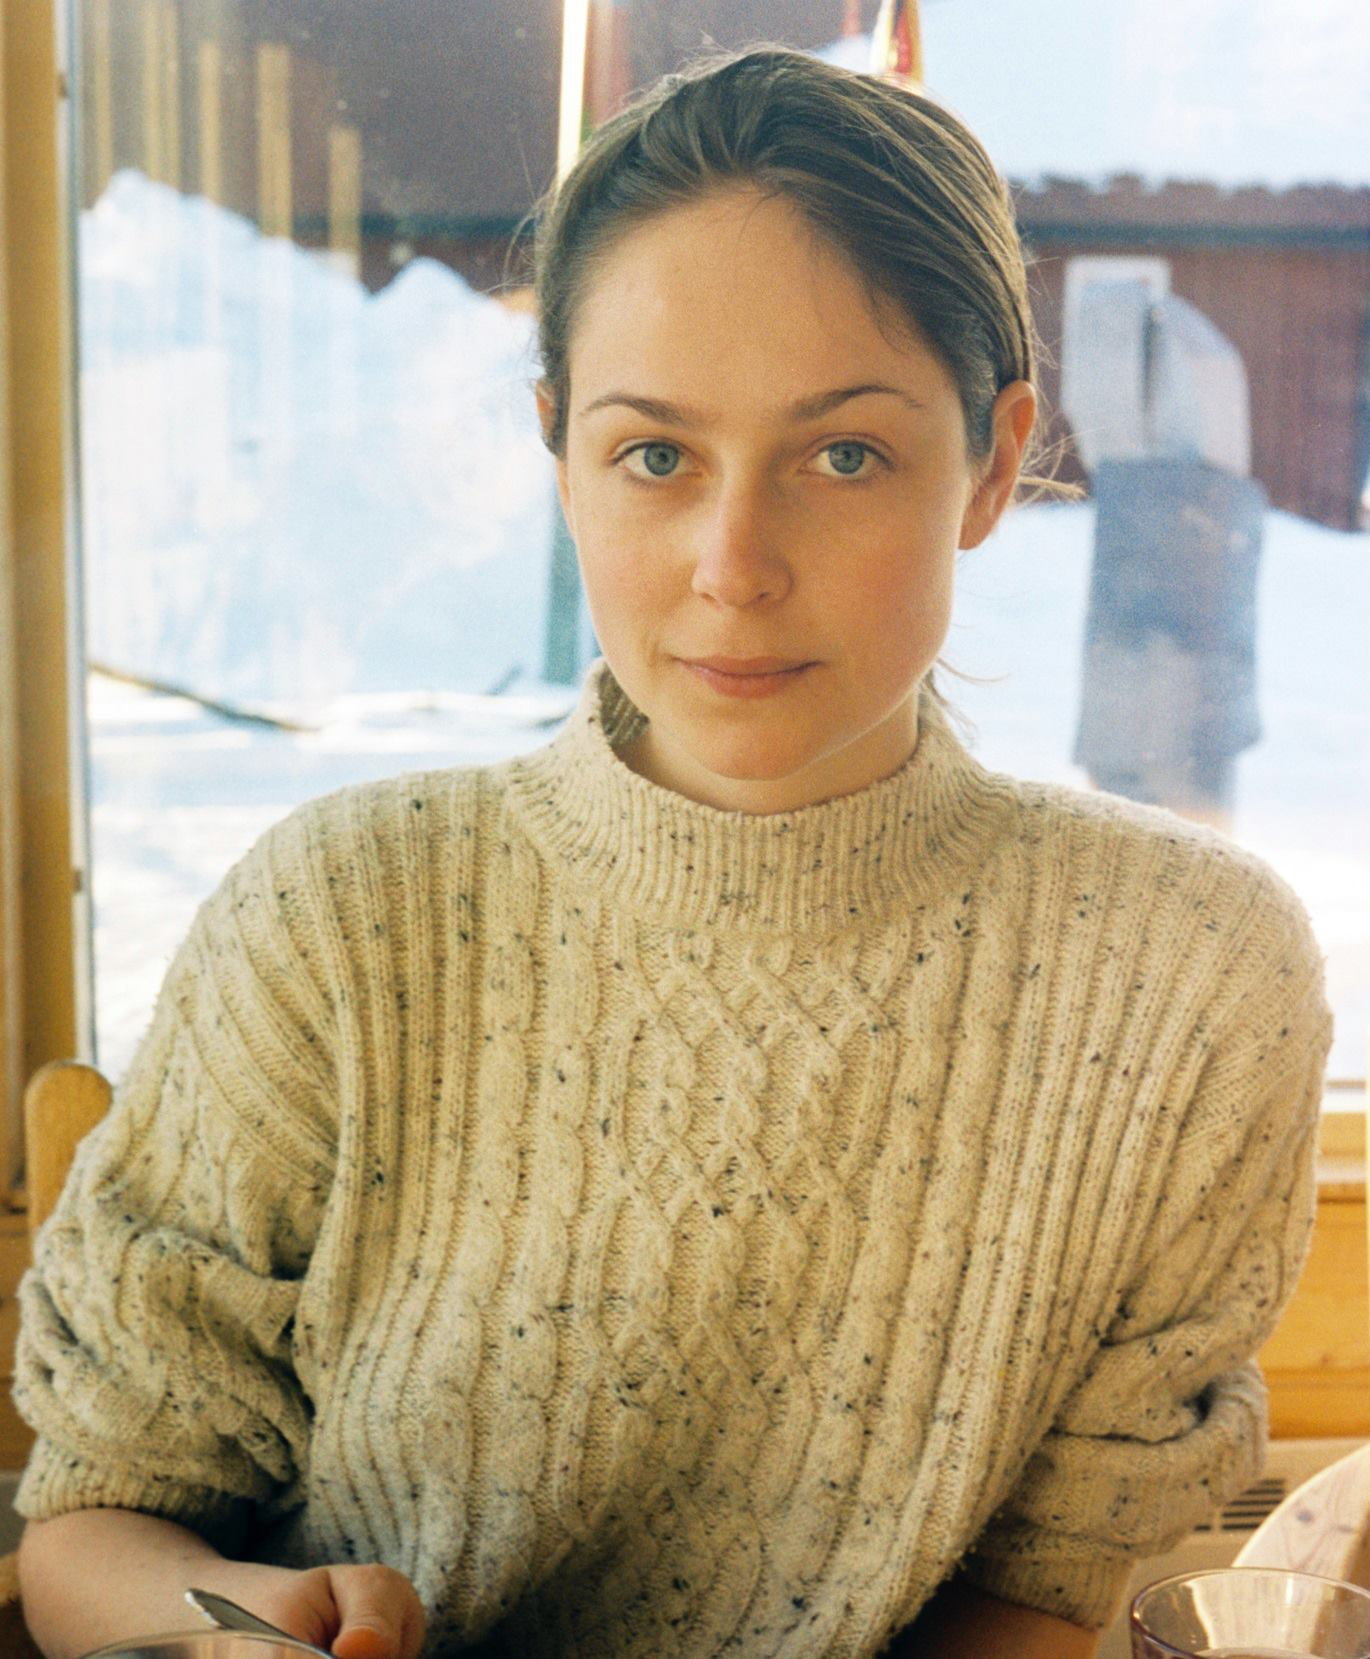
\includegraphics[width=0.13\linewidth]{Nikkaluokta} & 
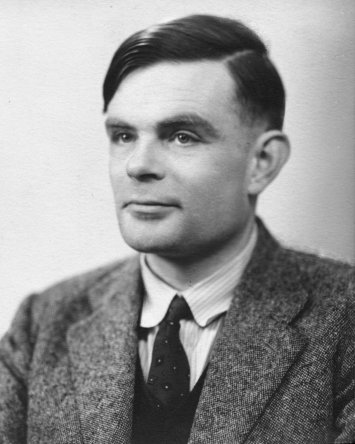
\includegraphics[width=0.13\linewidth]{Alan_Turing_photo} & 
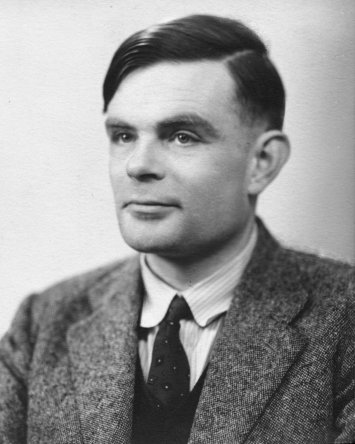
\includegraphics[width=0.13\linewidth]{Alan_Turing_photo} & 
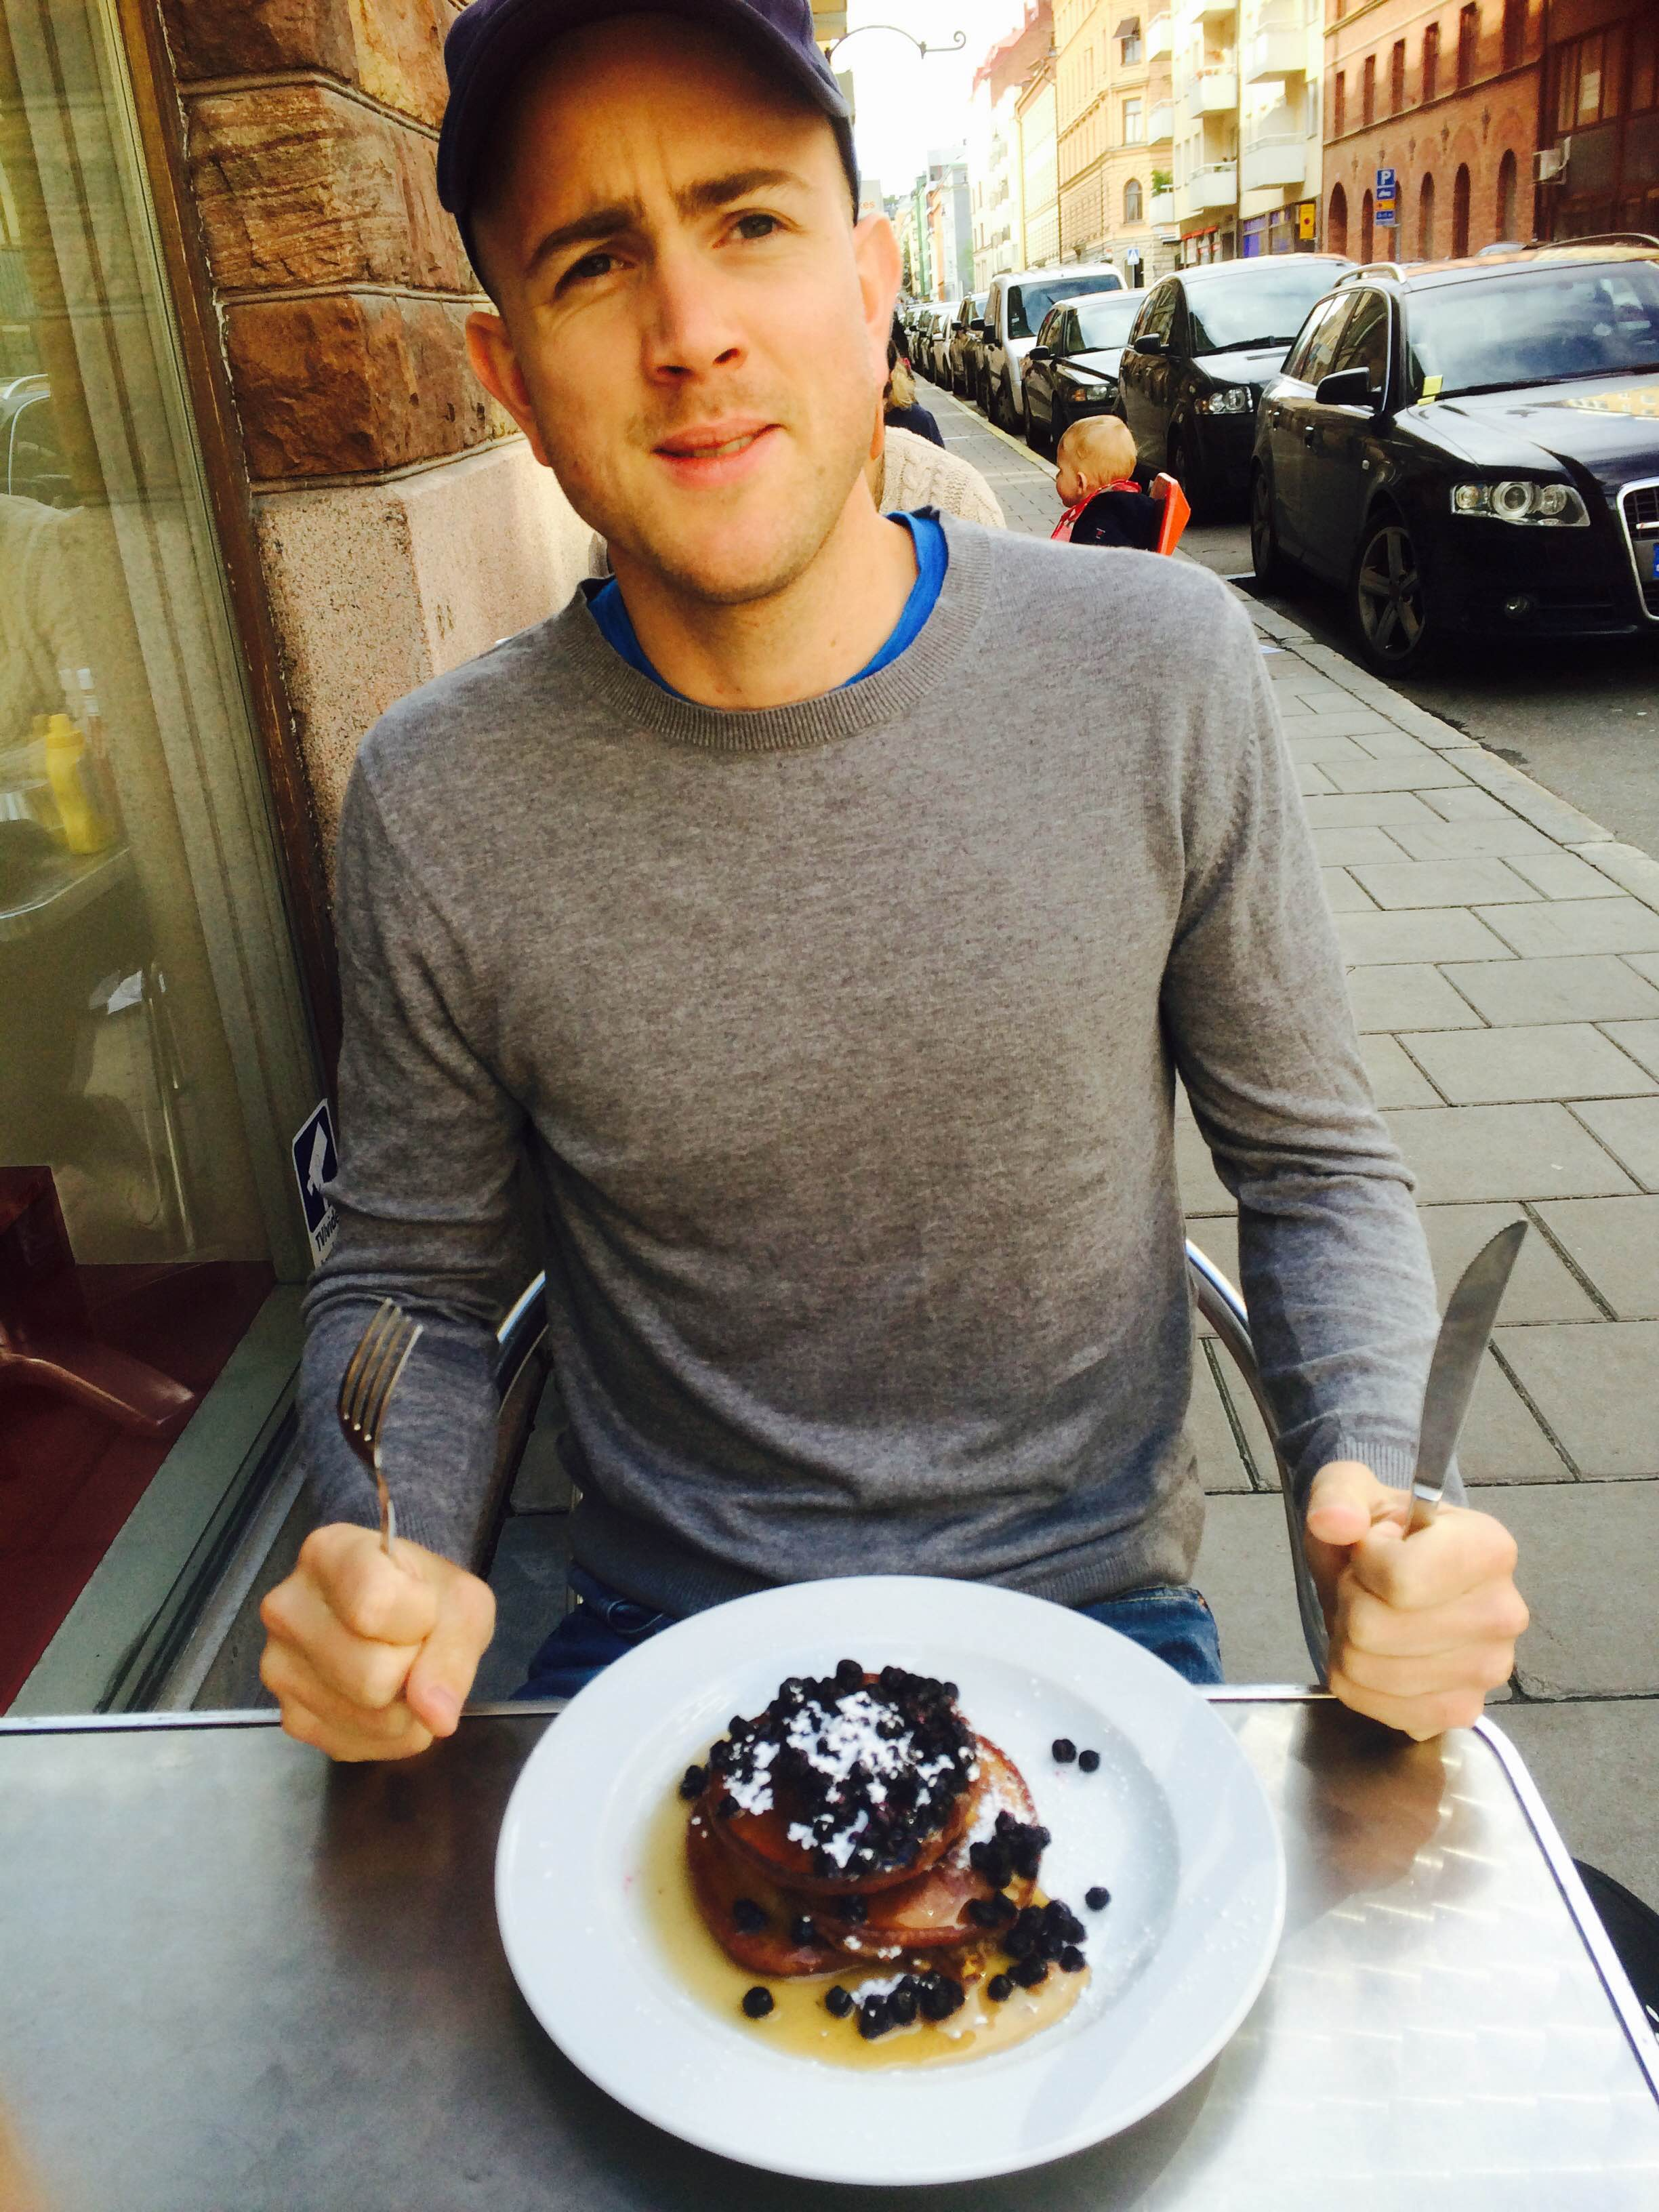
\includegraphics[width=0.13\linewidth]{erikpancakes}
\end{tabular}} 
% Normally there will not be any pictures but we want
% these so that we can connect faces to names in the course
% We also want birthdates so that we can tell people with the same
% name apart
\date{}

\pagestyle{fancy}
\setlength{\headheight}{15pt}
\fancyhf{}
\cfoot{\thepage / \pageref{LastPage}}
\lhead{DD2380 ai15} % DO NOT REMOVE!!!!
\rhead{S. Broom\'e, J. Krebs, V. Geffrier, E. Fredriksen} %% UPDATE WITH YOUR NAMES

\begin{document}

\maketitle
\thispagestyle{fancy}

\begin{abstract}
An investigation of how basic n-gram models of our own implementation can be improved by adding smoothing techniques and grammar constraints. Tests have been performed on corpora of varying character.
\end{abstract}



\clearpage

%%%%%%%%%%%%%%%%%%%%%%%%%%%%%%%%%%%%%%%%%%%%%%%%%%%%%%%%%%%%%
%%%%%%%%%%%%%%%%%%%%%%%%%%%%%%%%%%%%%%%%%%%%%%%%%%%%%%%%%%%%%
\section*{NOTE}
\begin{itemize}

\item The following sections are arranged in the order they would appear in a scientific paper. We think that these sections need to be there and written. However, these are only guidelines and if you think that some of these sections or subsections are irrelevant to you, please feel free to remove them. Similarly, if you want to include more sections or subsections please go ahead. Also feel free to rearrange them according to your convenience, but keeping some common sense (eg.~Introduction cannot come after Conclusions).

\item \textit{Introduction, Related Works, Experimental Results, Discussions, Summary} are sections that MUST be contained.

\item In the section of your \textit{Method}: please do not list your project as log book entries, please talk about the final method you want to present to us. Talk about the method scientifically or technically and not as "I did this..." "Then I tried this..." "this happened...." etc.

\item Do not paste any code unless it is very relevant!

\item The section \textit{Contributions} is a place to express any difference in contributions. The default assumption is that you all agree that all of you had an equal part to play in the project.

\item We suggest that you try to write this as scientifically as possible and not simply like a project report. Good Luck!

\item Please remove \textbf{this} NOTE section in your final report.

\end{itemize}
\section{Introduction}
\label{sec:intro}

Being able to dissect, classify, analyze and reproduce language is a highly relevant task for various fields. In the realm of artificial intelligence, we want to give language to our agents by means of communicating with them. When we deal with natural language processing we say that we make language models. Seen as there is no finite set of rules that can describe, say, the entire English language in a complete sense, for pragmatic reasons our best option seems to be basing our models on probabilistic observations - regardless of Noam Chomsky's contempt\cite{JurafskyBook} for the notion of probability of a sentence.

At the foundation of every language model that wants to predict words is the concept of n-grams, a method based on probabilistic distributions over length n combinations of subsequent words. An n-gram is a Markov chain of degree n-1. This quite simple construct can capture many patterns in sentences. Even though it doesn't consider grammar explicitly, grammar will inevitably be built in. For instance, an adjective will in many cases be followed by a noun, or a pronoun by a verb, and thus a bigram composed of those two grammatical types in the mentioned order will score high in probability. 

An n-gram gives us context for words, albeit not the full one. Gao and Suzuki\cite{gao2004long} explore long distance dependency for words through word clusters and the linguistically motivated {\it function word skipping} method where function words such as "has", "a", "in", "and", "the", etc, are skipped in favor of more significant words, called head words. In our experiments however, we will not delve further into this subject.

N-grams can also be used in a meta-sense - for instance it's common for part-of-speech-taggers to use n-gram models where they tag the current word based on the last word's tag.

There are some practical issues with the classical n-gram model. What do we do with the n-grams that aren't in our training set and thus have zero probability assigned? This is where techniques of so called smoothing comes in so that our model doesn't fail upon encountering a previously unseen word in the test set. And in case we are dealing with a higher-order n-gram and we find it has no probability mass , we might want to "back off" from the higher order and estimate the probability for a conditioned unigram, meaning we temporarily look at a smaller portion of a word's history.

Furthermore, what kinds of test sets does our training set allow us to perform well on? One should train on a  corpus which is representative of the domain of the intended use. And what happens to our model when we apply it to languages with a higher degree of inflection like Swedish, Basque or German?

From the above examples we see that in many cases just using the n-gram model in itself will not suffice. Over the years, researchers in natural language processing have added a lot of tweaks to the original idea such as linear combinations of n-grams, cache language models, LSA-based language models and maximum entropy models, to name a few.

In what follows we will explore n-gram models of varying degrees on dito corpora and grammar to see which results are obtained under which circumstances.

\subsection{Related works}
We began our exploring of natural language processing through the Natural Language Toolkit website and the accompanying book, Natural Language Processing with Python. The theory to accompany the more practical methods from NLTK was mainly obtained from Daniel Jurafsky and James H. Martin's 1999 book Speech and Language processing \ref{JurafskyBook}. Daniel Jurafsky also has made a series of video lectures on the subject for a Coursera online course. From \ref{brown1992} and \ref{garay2006text} we got a sense of the challenges of extending the concept of n-grams, as well as for modern applications of text prediction.

\subsection{Outline}
The lion's share of the report consists of three sections, hereunder, concerning respectively n-gram models, n-gram models with smoothing and n-gram models with grammar constraints, where each of them contains some theory, accounts of our related experiments and discussions of possible issues. In the end, the results of our work are presented with a subsequent summary and conclusion.

%%%%%%%%%%%%%%%%%%%%%%%%%%%%%%%%%%%%%%%%%%%%%%%%%%%%%%%%%%%%%
%%%%%%%%%%%%%%%%%%%%%%%%%%%%%%%%%%%%%%%%%%%%%%%%%%%%%%%%%%%%%
%%%%%%%%%%%%%%%%%%   NGRAM MODELS   %%%%%%%%%%%%%%%%%%%%%%%%%
%%%%%%%%%%%%%%%%%%%%%%%%%%%%%%%%%%%%%%%%%%%%%%%%%%%%%%%%%%%%%
%%%%%%%%%%%%%%%%%%%%%%%%%%%%%%%%%%%%%%%%%%%%%%%%%%%%%%%%%%%%%
\section{N-gram models}
\label{sec:ngram}

\subsection{Theory}
The first mathematical tool needed in all natural language processing experiment is n-gram models. Speech taggers, smoothing and other methods may not be implemented at first, but n-gram models are needed to predict the next likely words of a sentence.

These models are quite easy to understand: if n is a fixed integer, a n-gram model works as a Markov chain to predict the next word. A model is trained on a corpora C, for instance a book or a set of books, so that the probability of each n-gram in the language is learned by the model. The bigger the corpora the more accurate and reliable will be the model as it will have more data to compute probabilities of sequences. More precisely, the probability $p$ that the word $w_n$ follows the group of words $w_1 w_2 ... w_{n-1}$ is given by the following formula:

$$ p = p(w_n | w_1 .. w_{n-1}) = \frac{|{(w_1, .., w_{n-1}, w_n) \in C}|}{|{(w_1, .., w_{n-1}, x) \in C}|} $$

With this formula, it is possible to know the more likely next word of a sentence, but also to generate the end of the sentence, each new word selected at random using this probability distribution. Therefore, a n-gram which appeared a lot in a corpora is more likely to appear in the sentence generator. However, this also tells us that heuristically, we should expect different results from one corpora to another. For instance using corpora from Shakespeare, the generated sentences are likely to be more erratic than with a novel since Shakespeare's syntax and grammar are more complicated. For modernist poetry like Whitman's Leaves of Grass (corpus \# 4) it turns out to work quite well with a basic n-gram model, since the somewhat abstract resulting sentences fit with the textual situation and since the verse structure isn't as demanding as in shakespearian texts. Poetry has higher context satisfaction for a crude n-gram model.

\subsection{Experiments}
\subsubsection{Parameter $n$}
	The first experiment we did was to try to understand the influence of n in our word predictor and how we could tune this parameter. In these experiments, only the corpora and n is changed - no parts of speech tagger or smoothing have been used. The table \ref{tab:corpus2} shows multiple iterations of prediction of the end of the sentence "Alice was looking for" with n-gram models for n between 1 and 4. The corpora used was the novel "Alice in Wonderland" from Lewis Carroll, 1865. 
	
We should note that a 1-gram model is not a Markov model. It just predicts a word according to its frequency in a book, regardless of the previous words. As punctuation symbols are considered as words in this corpora, that explains why it predicts so many commas and apostrophes. 

A 2-gram model will only predict a word according to the immediately preceding word in the sequence. This explains why after words like "the" and "a" there are often adjectives or nouns. However, the prediction is still not perfect because of the short reach of a 2-gram model.

With 3-gram models and 4-gram models one can see that the sentences are a bit more grammatically correct but there is still some issues since the English grammar and syntax are not used in these models. This is why this is necessary to implement taggers and use a model that takes into consideration the grammar and the syntax of a language. Another thing with 4-gram models is that we can see the predictions are quite close to each other for different attempts. This is because the more words are fixed, the less freedom there is for the next word: there are fewer bigrams starting with "for" than 4-grams starting with "was looking for" in the corpora.
	
If n is too low, the predictor will be inferior because one or two words might not be enough to predict a likely next word. However if n is too big, the corpora needs to be really extensive as well and contain enough different n-gram so that the predictor is more diversified.

\subsubsection{The corpora}
See \ref{tab:corpora1} for a table of our tested corpora.
\begin{table}
\begin{center}
\begin{tabular}{|c|l|c|c|}
\hline
\# & Tested corpora & Year & Nr. of words\\ \hline
1 & Selected poems by William Blake & 1789 & 8354 \\ \hline
2 & Alice's Adventures in Wonderland by Lewis Carroll & 1865 & 34110 \\ \hline
3 & The Bible & & 100000 (1010654) \\ \hline
4 & Leaves of Grass by Walt Whitman & 1891 & 154883\\ \hline
5 & Moby Dick by Herman Melville & 1851 & 260819\\ \hline


\end{tabular}
\caption{The corpora tested in the n-gram experiments.}
\label{tab:corplist}
\end{center}
\end{table}

\subsubsection{Example results}

\begin{table}
%\begin{center}
\begin{tabular}{| l |c|}
\hline
Query followed by 10 generated words & $n$ \\ \hline
"Infant smiles are his own . Gone was thy Maker lay . Pretty joy to " & 2\\ \hline
"Infant smiles are his own destruction ? Can delight . Folly is dwelling too ?"& 2 \\ \hline
"Infant smiles are his own smiles on my foe outstretched beneath the skies ; And" & 2 \\ \hline
"Infant smiles are his own grave plot she in darkness plough ? Can a threat" & 2 \\ \hline
"Infant smiles are his own destruction ? When we rose to tenfold life , merrily" & 2 \\ \hline

"Infant smiles are his own smiles ; Heaven and earth to peace beguiles . DIVINE " & 3 \\ \hline
"Infant smiles are his own smiles ; Heaven and earth to peace beguiles . DIVINE" & 3 \\ \hline
"Infant smiles are his own smiles ; Heaven and earth to peace beguiles . DIVINE" & 3 \\ \hline
"Infant smiles are his own smiles ; Heaven and earth to peace , and fled " & 3 \\ \hline
"Infant smiles are his own smiles ; Heaven and earth to peace beguiles . DIVINE" & 3 \\ \hline

"Infant smiles are his own smiles ; Heaven and earth to peace beguiles . DIVINE" & 4 \\ \hline
"Infant smiles are his own smiles ; Heaven and earth to peace beguiles . DIVINE" & 4 \\ \hline
"Infant smiles are his own smiles ; Heaven and earth to peace beguiles . DIVINE" & 4 \\ \hline
"Infant smiles are his own smiles ; Heaven and earth to peace beguiles . DIVINE" & 4 \\ \hline
"Infant smiles are his own smiles ; Heaven and earth to peace beguiles . DIVINE" & 4 \\ \hline
\end{tabular}
\caption{ Corpus 1}
\label{tab:corpus1}
%\end{center}
\end{table}

\begin{table}
%\begin{center}
\begin{tabular}{| l |c|}
\hline
Query followed by 10 generated words & $n$ \\ \hline
"Alice was looking for a very neatly spread his belt and began . ' " & 2\\ \hline
"Alice was looking for eggs , I can kick a little bottle that stood "& 3 \\ \hline
"Alice was looking for the fan and a pair of white kid gloves , " & 4 \\ \hline
\end{tabular}
\caption{Corpus 2}
\label{tab:corpus2}
%\end{center}
\end{table}

\begin{table}
%\begin{center}
\begin{tabular}{| l |c|}
\hline
Query followed by 10 generated words & $n$ \\ \hline
"And they were both naked unto Pharaoh ' s milk , and shut him . " & 2\\ \hline
"And they were both naked ? 26 And Miriam the flesh from thence did Sarah"& 2 \\ \hline
"And they were both naked ? what hast done in the best of the north" & 2 \\ \hline
"And they were both naked , I have established by my master saw that he" & 2 \\ \hline
"And they were both naked ; and daubed it without blemish unto him : 13" & 2 \\ \hline

"And they were both naked , the people , and Calneh , in the coupling " & 3 \\ \hline
"And they were both naked , the face of the burnt offering , even the" & 3 \\ \hline
"And they were both naked , the children of Israel , and the sheep ." & 3 \\ \hline
"And they were both naked , the camels had done to him as before ." & 3 \\ \hline
"And they were both naked , the God of thy servants it be for a" & 3 \\ \hline

"And they were both naked , the man that brought us up out of the" & 4 \\ \hline
"And they were both naked , the man is become as one of the Hebrews" & 4 \\ \hline
"And they were both naked , the man is become as one of them opened" & 4 \\ \hline
"And they were both naked , the man that brought us up out of that" & 4 \\ \hline
"And they were both naked , the man and his household came with Jacob ." & 4 \\ \hline

\end{tabular}
\caption{ Corpus 3}
\label{tab:corpus3}
%\end{center}
\end{table}

\begin{table}
%\begin{center}
\begin{tabular}{| l |c|}
\hline
Query followed by 10 generated words & $n$ \\ \hline
"The delicious singing of the mother ' d ship - clad soldiers of ooze and what" & 2\\ \hline
"The delicious singing of the mother ' d eve delicious word , Elements merge with the"& 2 \\ \hline
"The delicious singing of the mother ' d back on the midst of Nature your tongue" & 2 \\ \hline
"The delicious singing of the mother kisses of the clasp me shall cover ' s funeral" & 2 \\ \hline
"The delicious singing of the mother told - lung ' d every blow through the same" & 2 \\ \hline

"The delicious singing of the mother to part , and the climbing sap , Arms and" & 3 \\ \hline
"The delicious singing of the mother sleeps with at night , The singers of old or" & 3 \\ \hline
"The delicious singing of the mother misused by her children , resolute , under the sun" & 3 \\ \hline
"The delicious singing of the mother never turning her vigilant eyes ,) Calmly a lady '" & 3 \\ \hline
"The delicious singing of the mother of many nations , the shelves are crowded with perfumes" & 3 \\ \hline

"The delicious singing of the mother shines on the white wrist of the daughter , The" & 4 \\ \hline
"The delicious singing of the mother , the Mississippi flows , Of mighty inland cities yet" & 4 \\ \hline
"The delicious singing of the mother of many children , These clamors wild to a race" & 4 \\ \hline
"The delicious singing of the mother , or of me ; Of their languages , governments" & 4 \\ \hline
"The delicious singing of the mother shines on the white wrist of the daughter , The" & 4 \\ \hline

"Sing on there in the swamp - congratulatory signs and dead . I shall never refuses" & 2\\ \hline
"Sing on there in the swamp in songs , English war , Sunlight by the Cascade"& 2 \\ \hline
"Sing on there in the swamp - dug in disgrace to give an open air I" & 2 \\ \hline
"Sing on there in the swamp , busier sphere more in granite walls of the West" & 2 \\ \hline
"Sing on there in the swamp in vain the country ; You past .) Now I" & 2 \\ \hline

"Sing on there in the swamp in the houses are alive with people , I pause" & 3 \\ \hline
"Sing on there in the swamp in secluded recesses , From the head of the real" & 3 \\ \hline
"Sing on there in the swamp - cedars , with muttering thunder and lambent eyes watch" & 3 \\ \hline
"Sing on there in the swamp in the ranks marching , on I go , I'" & 3 \\ \hline
"Sing on there in the swamp - perfume , with brow elate and governing hand ." & 3 \\ \hline

"Sing on there in the swamp , O singer bashful and tender , I hear in" & 4 \\ \hline
"Sing on there in the swamp , O singer bashful and tender , I hear the" & 4 \\ \hline
"Sing on there in the swamp , O singer bashful and tender , I hear the" & 4 \\ \hline
"Sing on there in the swamp , O singer bashful and tender , I hear in" & 4 \\ \hline
"Sing on there in the swamp , O singer bashful and tender , I hear the" & 4 \\ \hline

\end{tabular}
\caption{ Corpus 4}
\label{tab:corpus4}
%\end{center}
\end{table}


\begin{table}
%\begin{center}
\begin{tabular}{| l |c|}
\hline
Query followed by 10 generated words & $n$ \\ \hline
"However , there is a whale - fleet of this , and the two" & 2\\ \hline
"However , there is no place to live in the captain ' s a"& 3 \\ \hline
"However , there is no telling . But a day or two previous ," & 4 \\ \hline
"I think that you must have been offered a whale , when the long" & 2\\ \hline
"I think that you do yours in approved state stocks bringing in good time"& 3 \\ \hline
"I think that you really perceived drops of moisture in the spout - hole" & 4 \\ \hline
\end{tabular}
\caption{Corpus 5}
\label{tab:corpus5}
%\end{center}
\end{table}




\subsection{Issues}









\section{N-gram models with smoothing}

\subsubsection{Initial practical problems: an SRILM excursion}
Building a full-fledged language model in Python is not a trivial endeavor (this could be a project in itself). We thought NLTK provided the facilities to accomplish this, but it turned out this module had been deprecated due to bugs. 

SRI provides an extensive framework for just this task trough SRILM (this framework is also evidently widely adopted - the introductory SRILM article by Andreas Stolcke has over 3 000 Google Scholar citations). 

SRILM itself is a library of C++ classes, but contains ready-made command line tools. For example, invoking "ngram-count" on the Moby Dick corpus from NLTK (where corpus.txt has been parsed to match SRILMs format: one sentence per line with tokens separated by whitespace) produces an ngram language model of this text, with Good-Turing discounting and Katz backoff for smoothing:

\begin{lstlisting}[language=bash]
  $ ngram-count -text corpus.txt -lm model.LM -order 3
     -write model.NGRAM
\end{lstlisting}


This model (model.LM) can then be queried and processed with command line tools like for example ngram,

\begin{lstlisting}[language=bash]
  $ ngram -order 3 -lm model.LM -ppl input.sent -debug 1 
\end{lstlisting}


which produces

\begin{lstlisting}[language=bash]
  $ reading 19313 1-grams 
  $ reading 118199 2-grams
  $ reading 19961 3-grams
  $ this is a sentence 1 sentences, 4 words, 1 OOVs
  $ 0 zeroprobs, logprob= -6.1645 ppl= 34.7636 ppl1= 113.458
\end{lstlisting}


where input.sent is a text file containing the line "this is a sentence", and the output is the log probability of this sentence according to our model.LM (the word "sentence" is not part of the vocabulary ? 1 OOV.)

Doing actual predictions with this framework proved to be a bit harder, we found a Python wrapper (pysrilm) that was supposed to provide this functionality, however, it was a Cython extension that needed to be compiled and linked against the SRILIM library. This did not work, so we returned to our own Python n-gram model to implement a smoothing method ourselves.

\label{sec:ngramsmoothing}

\subsection{Theory}
	The issue behind simple n-gram models is that the maximum likelihood estimate only consider n-grams in the corpora. That is, many n-grams are not considered by the model to have a probability strictly positive because there is sparsity in the data. However in most cases one does not want to give a probability of 0 to unseen event: an event that did not occur in the training data could occur in the test data. Smoothing methods are used to adapt the probability distribution so that unseen events have a probability greater than 0. There are different ways of smoothing and we experimented mainly three methods implemented in $nltk$:
	
	\begin{description}
		\item[Witten-Bell:] This method gives the same probability mass to the unseen events as the probability mass of the events seen exactly once in the corpora. As there are usually a lot more unseen events than events that occured once, the model seems reliable because it will give a low probability to the unseen event. A parameter given is the number of total events, seen or unseen. If there are $m$ unique words in the corpora and we are considering n-grams, it is not necessarily $m^n$ since the corpora could be lacking words we want to add manually, or we can ignore some n-grams because they are not valid grammatically.
		\item[Lidstone:] This method simply adds a value $\gamma$ to all the frequency of events. It then computes the basic maximum-likelihood probability based on those new frequencies. This parameter, to tune, is usually around 0.5. In this case, this means the weight of an unseen event will become the third of the weight of an event that occured once. We can note that this method derives from the Laplace smoothing method which is when $\gamma = 1$.
		\item[Good-Turing:] This method is more complicated and gives to the events that occured $n$ times the same probability mass than the mass of the events that occured $n+1$ times. With high values of $n$ it can happen that no event occured that many times. For these events, an estimation is done. In the case of nltk, the number of events that occured $n$ times is estimated to be $N(n) = an^b$ where $a$ and $b$ are estimated using linear regression on the logarithm of the equation: $log N(n) = log a + b log n$.
		However, different methods can be used to estimate $N(n)$ when it equals $0$ in the corpora.
	\end{description}
	
	\subsection{Experiments}
	
	In the following experiments, we tried to point out how smoothing methods could change the probability distribution of the n-grams for our predictor. We also have compared the sentences with or without smoothing, but comparing the probability distribution makes more sense to understand how smoothing methods work. We also took a specific example with three n-grams of different frequencies in the corpora, to see how their probability and the ratio of their probability changes with the smoothing method.
	
\subsubsection{The probability distribution}
	As of figure \ref{fig:smoothingdist}, we tried to see the effect of the three methods mentionned earlier on the probability distribution of the 2-grams and 4-grams for the corpora "Alice in Wonderland". The n-grams with low frequency are not considered here as their probability is the same after smoothing with those methods. In blue is the probability distribution without smoothing and in red is the new probability distribution after a smoothing method. As we could expect, the latter is lower than the former because probability weight is given from seen events to unseen events. However, this mass is not the same for the different methods and the Lidstone probability for instance do not take the same weight from all n-grams. With the parameters tried, the Good Turing smoothing methods gives a distribution really close to the former, which is why the tuning of the parameters is important. It also depends on the size of the corpora as the ratio between the number of unseen events and seen events has a huge effect in the computation of the new probability distributions.

\begin{figure}
	\label{fig:smoothingdist}
	\begin{tabular}{cc}
		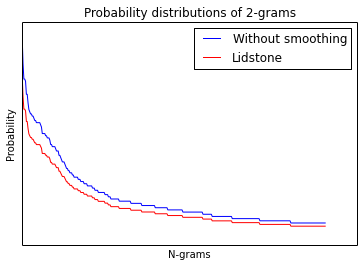
\includegraphics[width=0.52\linewidth]{2_Lidstone} & 
		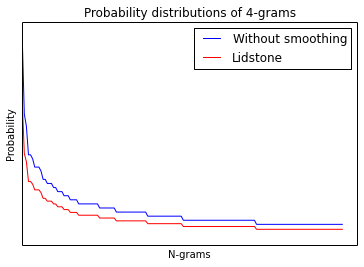
\includegraphics[width=0.52\linewidth]{4_Lidstone} \\
		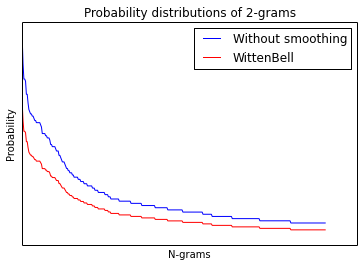
\includegraphics[width=0.52\linewidth]{2_WittenBell} & 
		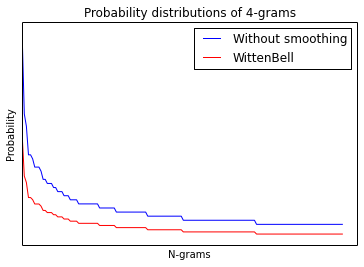
\includegraphics[width=0.52\linewidth]{4_WittenBell} \\
		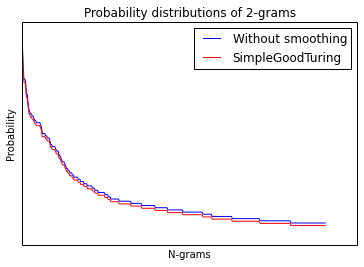
\includegraphics[width=0.52\linewidth]{2_Turing} & 
		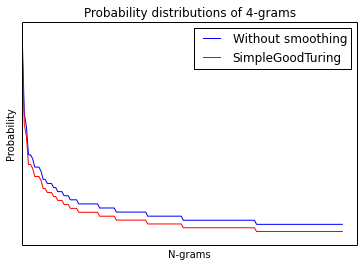
\includegraphics[width=0.52\linewidth]{4_Turing} \\
	\end{tabular}
	\caption{Changes of the probability distribution for different smoothing methods}
\end{figure}

\subsubsection{Specific example}
	Table \ref{tab:smoothingprobs} shows the evolution of the probabilities and ratio of the probabilities of three 3-grams in the same corpora. In the corpora, (she, was) has a frequency of 49, (she, is) has a frequency of 3 and (she, blue) is unseen. As we can seen, after smoothing technics, the probability of (she, blue) is not 0 anymore, which was expected. However we can see the ratio of the probabilities between (she, was) and (she, is) can change depending on the method. If Witten-Bell does not change it, Lidstone and Turing does as they do not allocate the same weight pourcentage of each seen events to the unseen ones.


\begin{table}[!h]
\centering
\caption{Data for different smoothing techniques}
\label{tab:smoothingprobs}
\begin{tabular}{@{}lllll@{}}
\toprule
Smoothing:     & None      & SGT       & WB        & LSPB 0.5   \\ \midrule
P(she, is)     & 8.795e-05 & 6.072e-05 & 6.025e-05 & 8.343e-05  \\
P(she, was)    & 0.001437  & 0.001396  & 0.0009841 & 0.001180   \\
P(she, blue)   & 0.000     & 3.701e-08 & 3.469e-08 & 1.192e-05  \\
Ratio was/is   & 16.33     & 22.99     & 16.33     & 14.14      \\
Ratio was/blue &           & 37710     & 28370     & 99.00      \\ \bottomrule
\end{tabular}
\end{table}

\subsection{Issues}
	The last example can show how careful one needs to be when it comes to smoothing. If the parameter is badly tuned, the probability of an unseen event such as (she, blue) can be great whereas it is not grammatically correct. This is why grammar constraints are needed to work with n-gram models, because simple models and smoothing technics cannot grasp the complex grammar and structure of a language.


\section{N-gram models with grammar constraints}
\label{sec:ngramgrammar}

\subsection{Theory}
\subsection{Experiments}
\subsubsection{The corpora}
\subsubsection{Example results}
\subsection{Issues}

%%%%%%%%%%%%%%%%%%%%%%%%%%%%%%%%%%%%%%%%%%%%%%%%%%%%%%%%%%%%%
%%%%%%%%%%%%%%%%%%%%%%%%%%%%%%%%%%%%%%%%%%%%%%%%%%%%%%%%%%%%%
\section{Summary and Conclusions}
\label{sec:summary}

N-gram models need additional layers consisting of smoothing techniques and grammar constraints to be more credible as  word predictors.


%%%%%%%%%%%%%%%%%%%%%%%%%%%%%%%%%%%%%%%%%%%%%%%%%%%%%%%%%%%%%
%%%%%%%%%%%%%%%%%%%%%%%%%%%%%%%%%%%%%%%%%%%%%%%%%%%%%%%%%%%%%
\section{Contributions}
\label{sec:contributions}
We the members of project groupXX unanimously declare that 
we have all equally contributed toward the completion of this
project. (PLEASE CHANGE THIS SUITABLY WITH DETAILS, IF IT IS NOT TRUE)


%%%%%%%%%%%%%%%%%%%%%%%%%%%%%%%%%%%%%%%%%%%%%%%%%%%%%%%%%%%%%
%%%%%%%%%%%%%%%%%%%%%%%%%%%%%%%%%%%%%%%%%%%%%%%%%%%%%%%%%%%%%


\bibliographystyle{plain}
\bibliography{reflist}



\end{document}
